En este apartado se va a explicar cómo se han implementado los requisitos tanto funcionales como no funcionales en la aplicación. 

\subsection{Home}

La pantalla principal o \textit{Home} recoge el requisito no funcional \textbf{RNF-1}, ya que tal como nos indica su propia descripción, se proporciona un sistema con interfaz de usuario.

En la esquina superior derecha se encuentra el botón \textit{Login}, en el cual, si es pulsado, redirige a la vista de inicio de sesión de usuario para diferenciar entre los sanitarios y los técnicos, tal y como nos indica el requisito funcional \textbf{RF-10}. Además, la aplicación es capaz de soportar el uso simultáneo de la misma por mínimamente dos usuarios, tal como dicta el requisito no funcional \textbf{RNF-4}.

\begin{figure}[H]
	\centering
	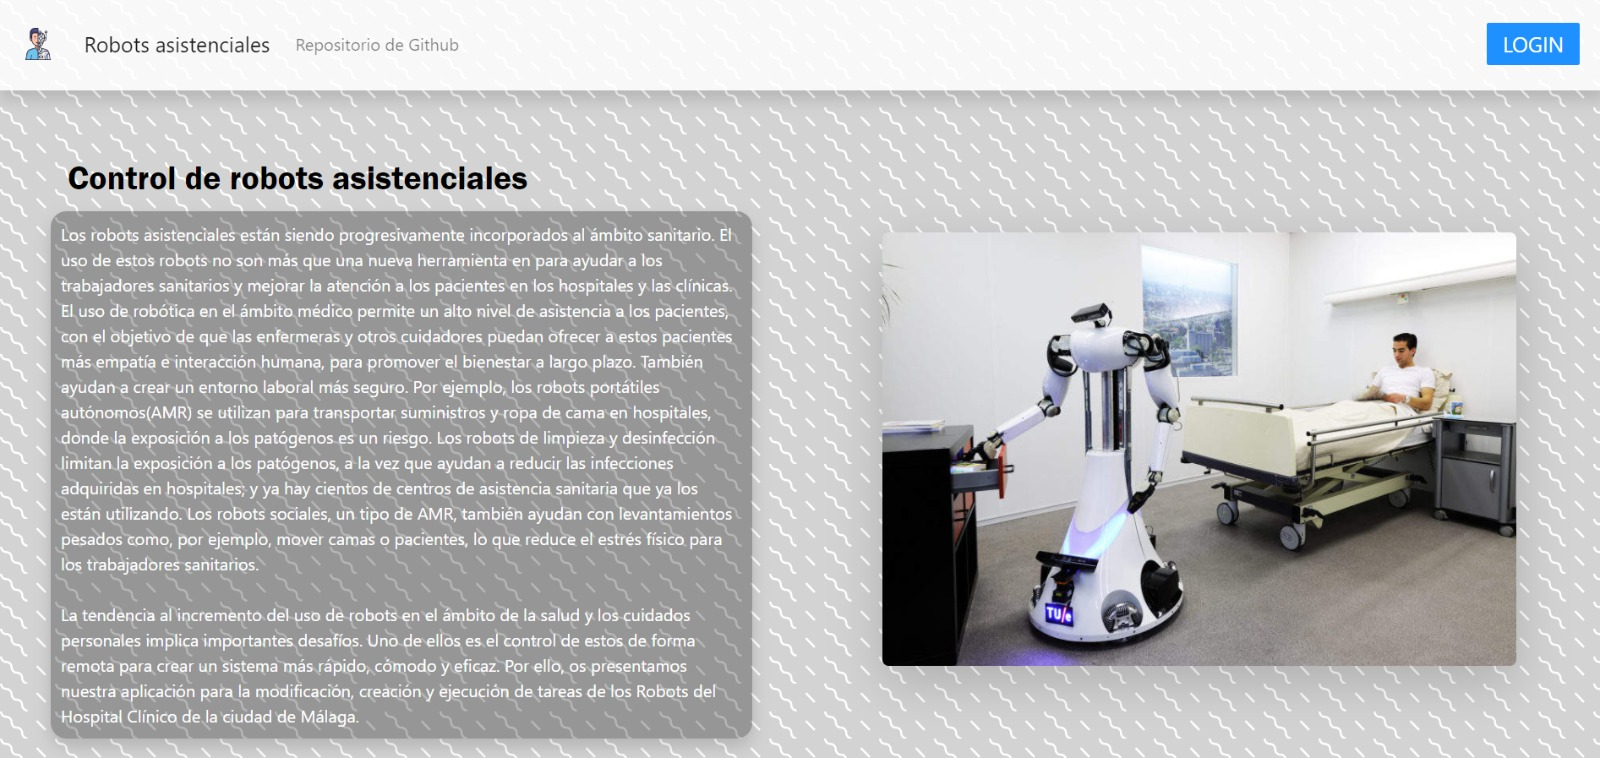
\includegraphics[width=1\textwidth]{images/Home.png}
	\caption{Home}
	\label{fig:UMLModel}
\end{figure}

\subsection{Vista de Médico}

Una vez que se ha iniciado sesión como sanitario, la aplicación nos redirige a la vista principal de este tipo de usuario, la cual está compuesta por un listado de tareas en una tabla encontrándonos con información de relevancia respecto a ellas como su tipo, el robot asignado, y el estado en el que se encuentra. 

\begin{figure}[H]
	\centering
	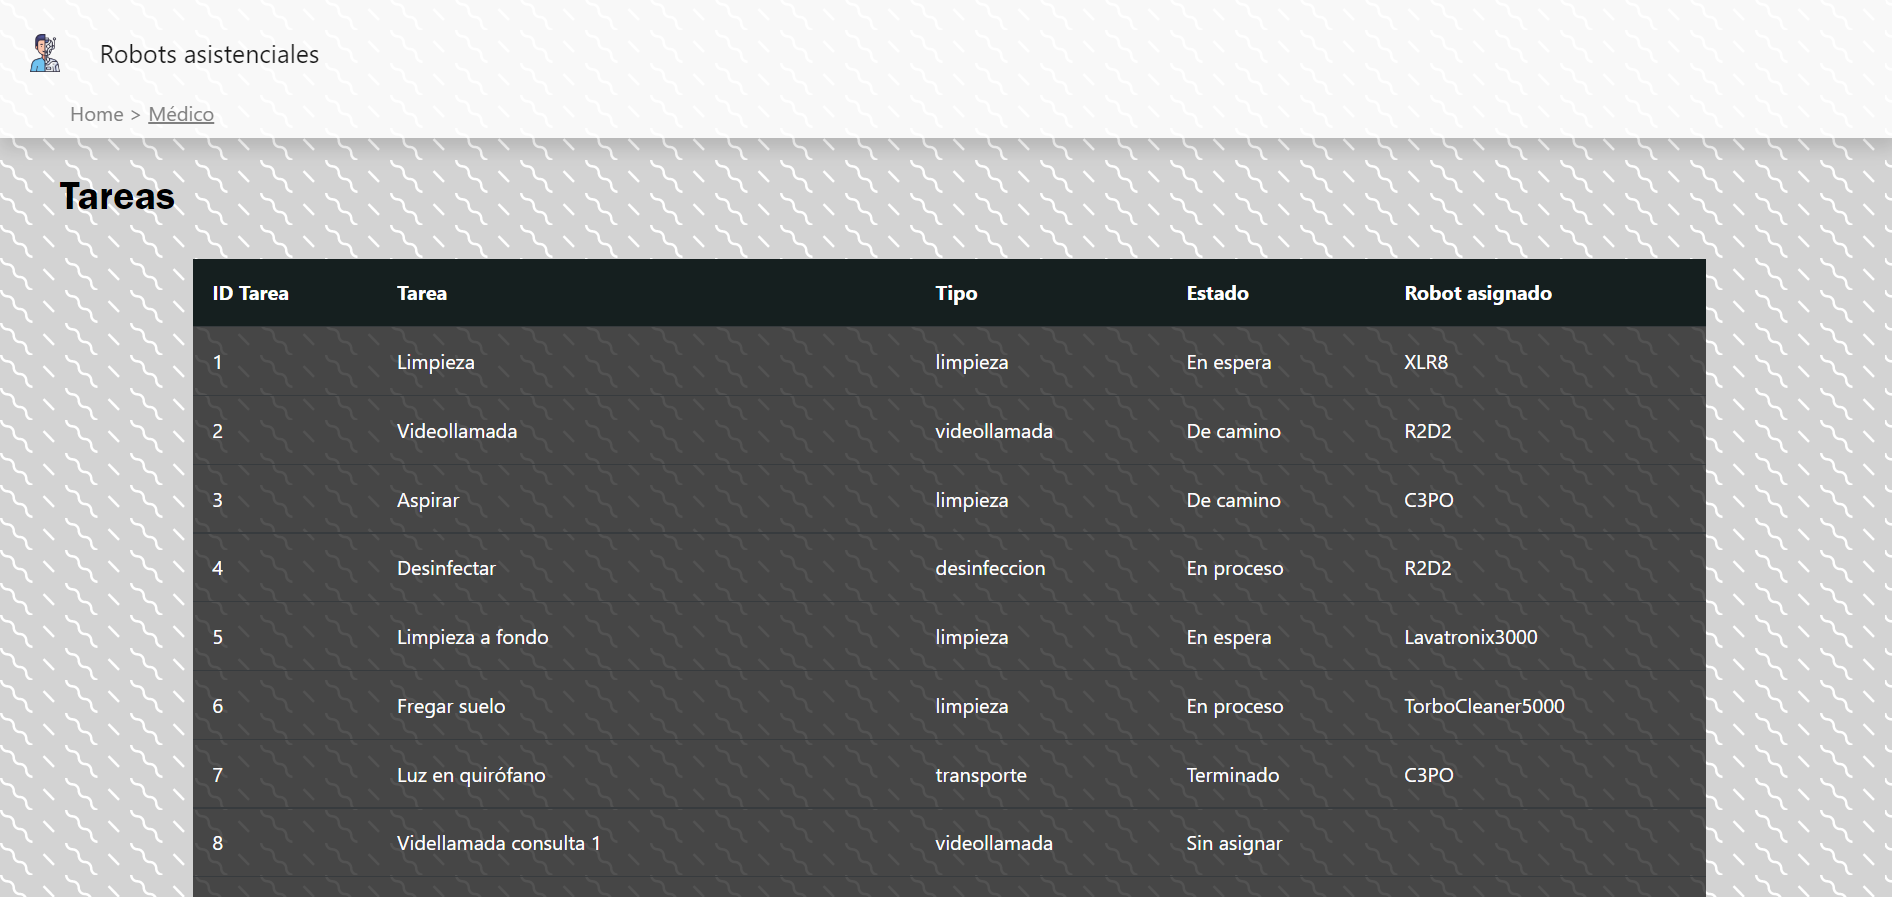
\includegraphics[width=1\textwidth]{images/VistaMedico.png}
	\caption{Vista Médico}
	\label{fig:UMLModel}
\end{figure}

Si seleccionamos una tarea, la aplicación nos redirige a una nueva vista, en la cual podemos asignarle un robot distinto o asignarle uno en caso de que esta no se encuentre asociada a ningún otro. A su vez, tenemos la opción de cancelar su ejecución cambiando su estado a "Sin asignar", además de cortar su asociación con el robot correspondiente. También, podemos asignar varias tareas a un mismo robot. Todo lo descrito anteriormente cumple con los requisitos \textbf{RF-1}, \textbf{RF-2}, \textbf{RF-7}, \textbf{RF-9}, \textbf{RNF-3} y \textbf{RNF-8}.

\begin{figure}[H]
	\centering
	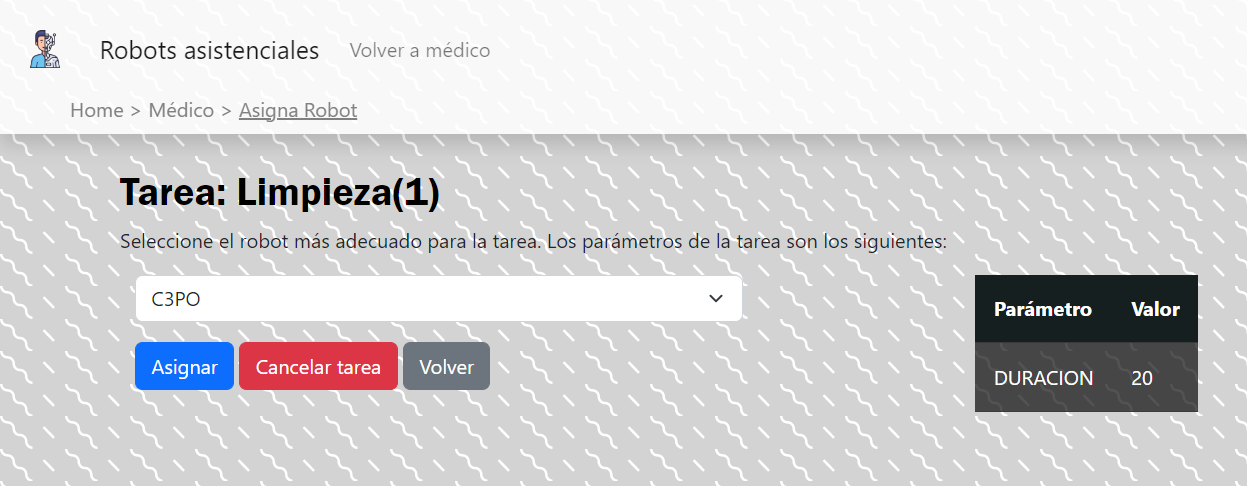
\includegraphics[width=1\textwidth]{images/VistaTarea.png}
	\caption{Vista Tareas}
	\label{fig:UMLModel}
\end{figure}

\subsection{Vista de Técnico}

Una vez que se ha iniciado sesión como técnico, la aplicación nos redirige a la vista principal de este tipo de usuario, la cual está compuesta por un listado de robots en una tabla encontrándonos con información de relevancia respecto a ellos como su ID, el nombre y las tareas que puede realizar cada uno. 
\begin{figure}[H]
	\centering
	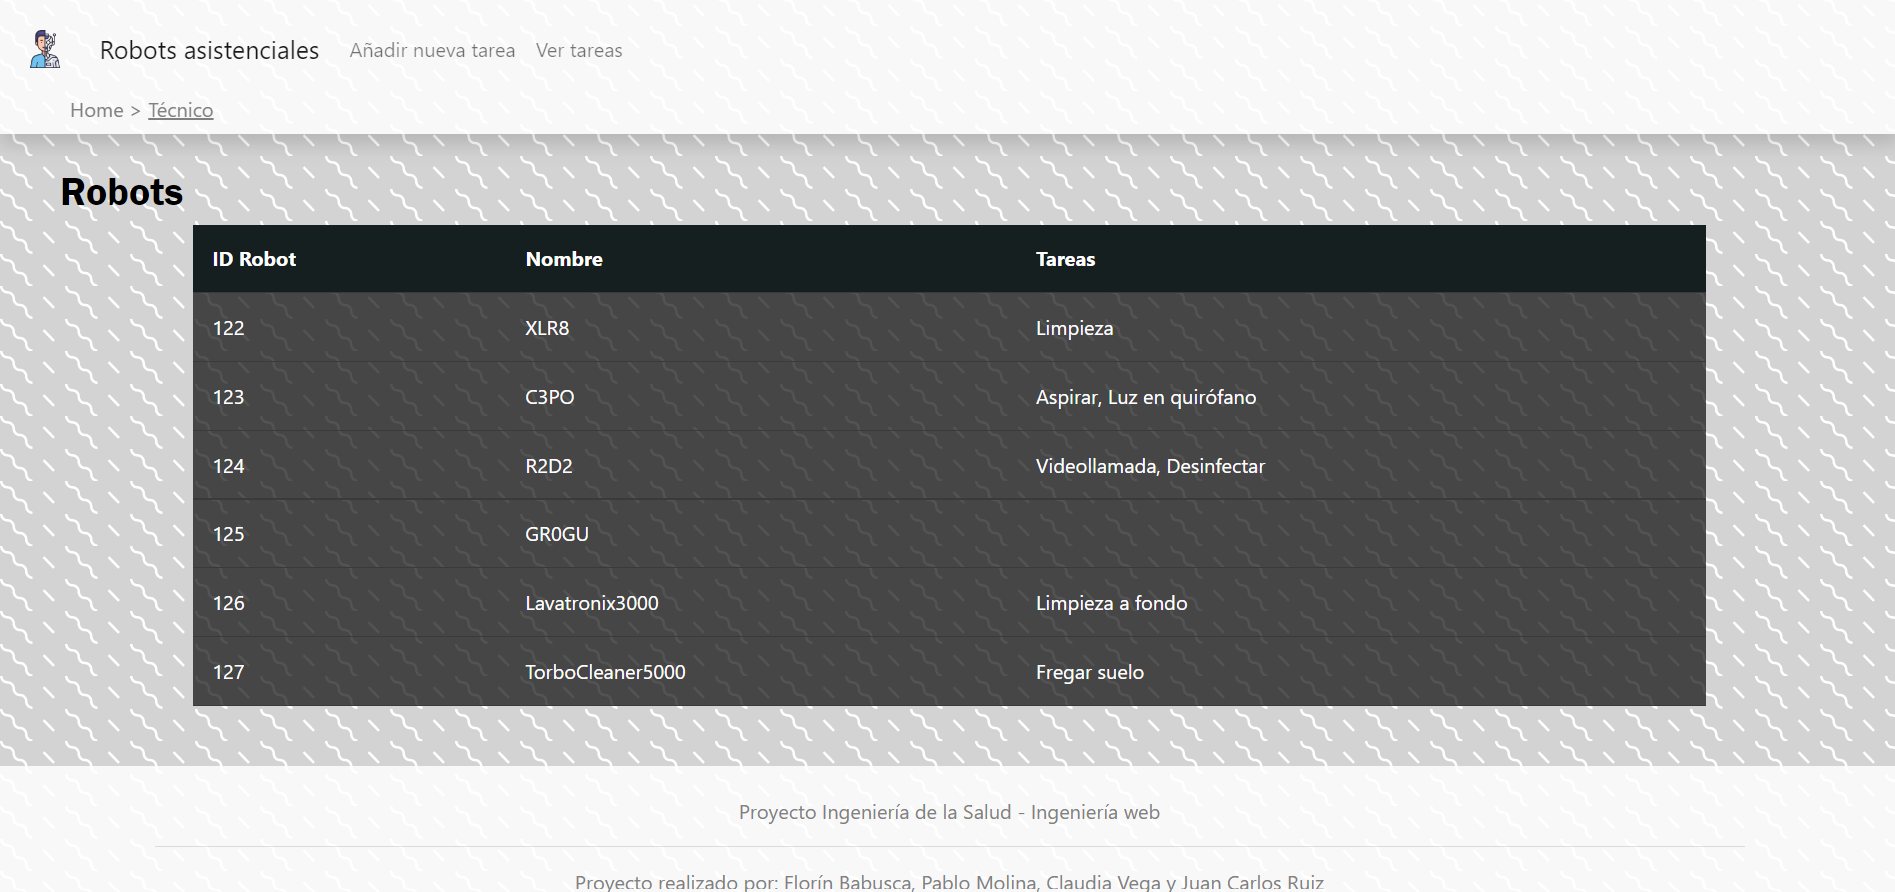
\includegraphics[width=1\textwidth]{images/VistaTecnico.png}
	\caption{Vista Técnico}
	\label{fig:UMLModel}
\end{figure}
En esta vista, tenemos la opción de crear un nuevo tipo de tareas, redirigiéndonos al siguiente pop-up en el que introduciremos el nuevo tipo de tarea deseado. 
\begin{figure}[H]
	\centering
	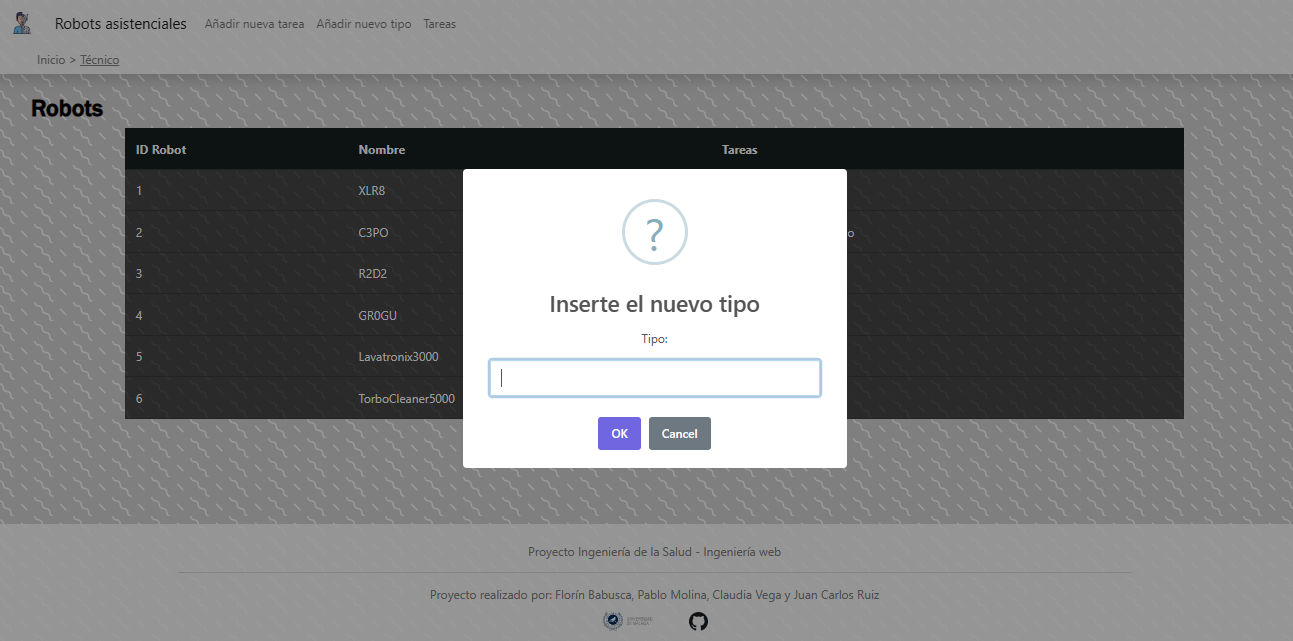
\includegraphics[width=1\textwidth]{images/NewRobotType.png}
	\caption{Nuevo tipo de robot}
	\label{fig:UMLModel}
\end{figure}

También, tenemos la opción de añadir una nueva tarea, la cual será de uno de los tipos de robots existentes.

\begin{figure}[H]
	\centering
	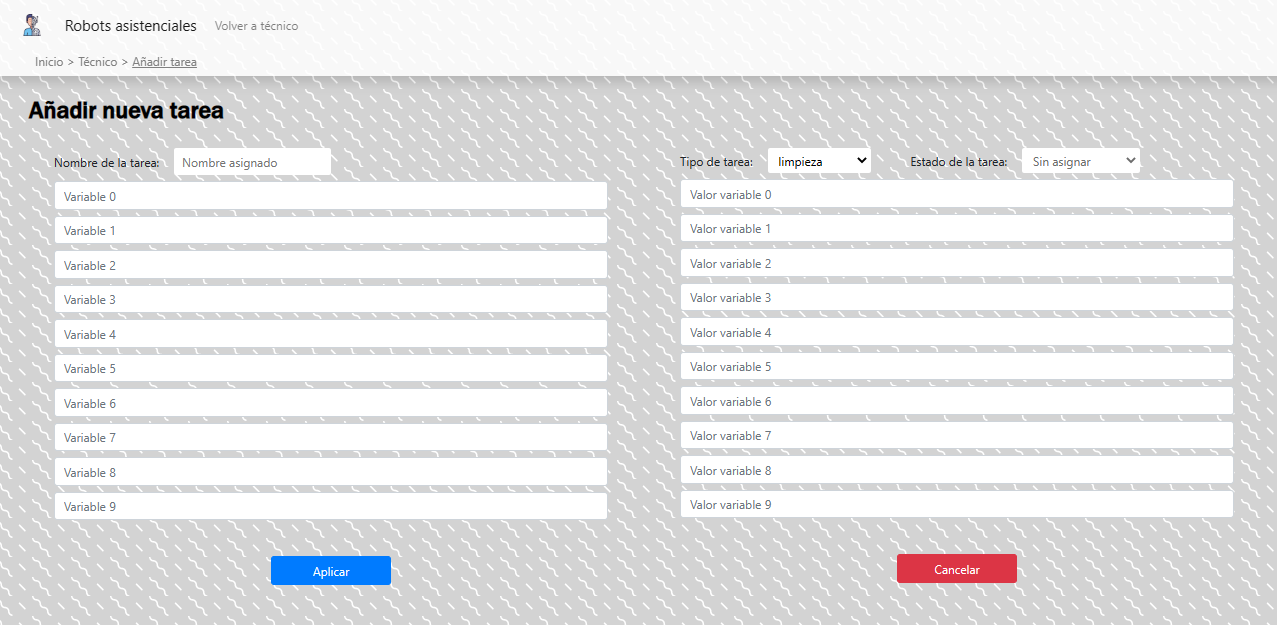
\includegraphics[width=1\textwidth]{images/Tech-TaskCreatorNoRobot.png}
	\caption{Nueva tarea sin robot asociado}
	\label{fig:UMLModel}
\end{figure}

Si seleccionamos un robot, la aplicación nos redirige a una nueva vista, en la cual podemos observar todas las tareas asociadas al robot elegido.
\begin{figure}[H]
	\centering
	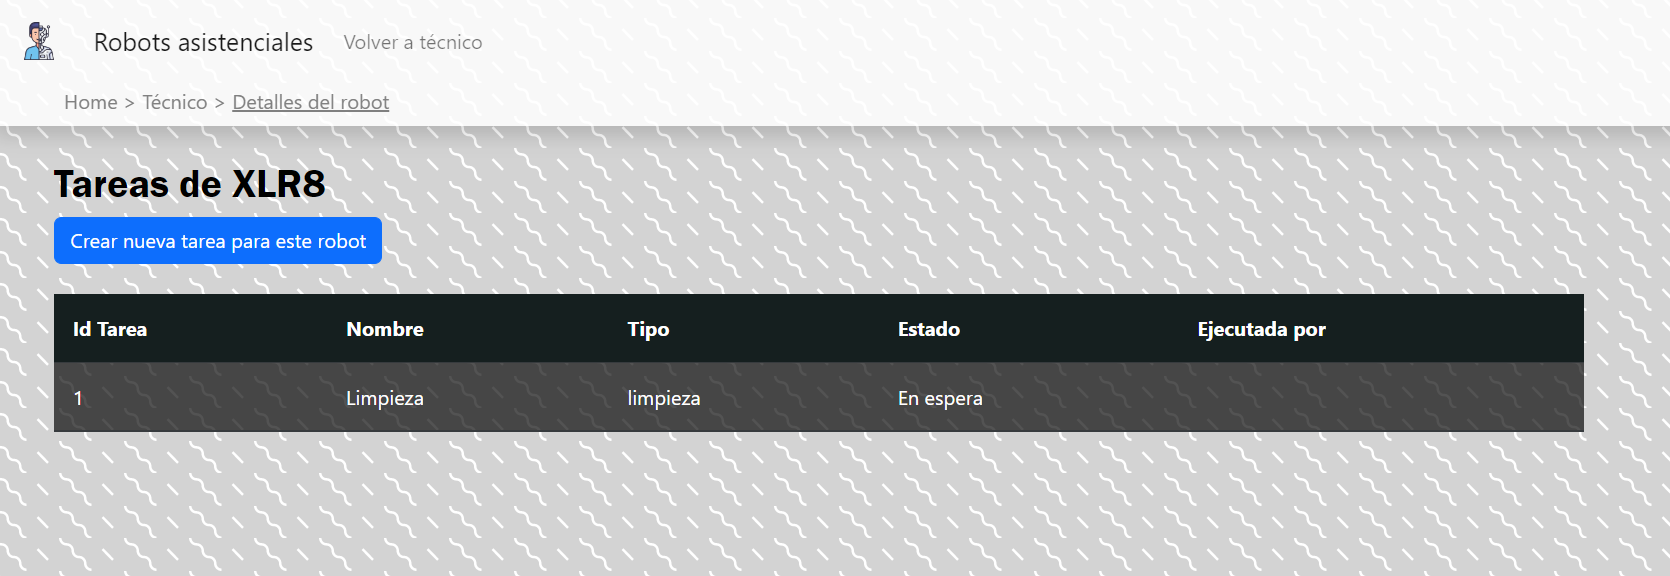
\includegraphics[width=1\textwidth]{images/CrearTareas.png}
	\caption{Tareas asociadas al robot elegido}
	\label{fig:UMLModel}
\end{figure}

A su vez, en esta vista podemos crear una nueva tarea para el robot que hayamos seleccionado. 
\begin{figure}[H]
	\centering
	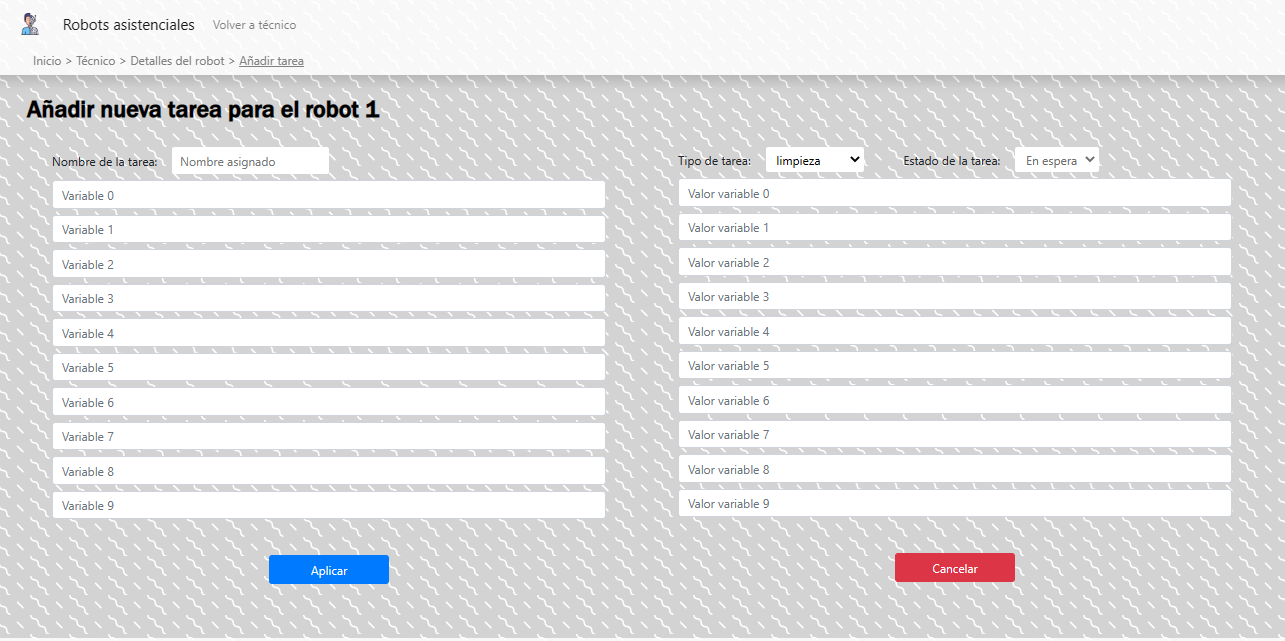
\includegraphics[width=1\textwidth]{images/TaskCreator.png}
	\caption{Creación de una nueva tarea}
	\label{fig:UMLModel}
\end{figure}


Lo anteriormente descrito cumple con los requisitos \textbf{RF-2}, \textbf{RF-6}, \textbf{RF-12}, \textbf{RF-13} y \\ 
\textbf{RNF-2}.

\subsection{Errores}

Por último, se ha implementado la posibilidad de que el robot notifique de algún tipo de error a la hora de realizar la tarea. Además, se ha hecho diferenciación de errores según la causa del problema. Por ejemplo, un error de sistema estará documentado si ha sido esa la causa, al igual que estará documentada la no realización de la tarea correspondiente por baja batería. Esto cumple con los requisitos \textbf{RF-4}, \textbf{RF-11} y \textbf{RNF-5}.

\begin{figure}[H]
	\centering
	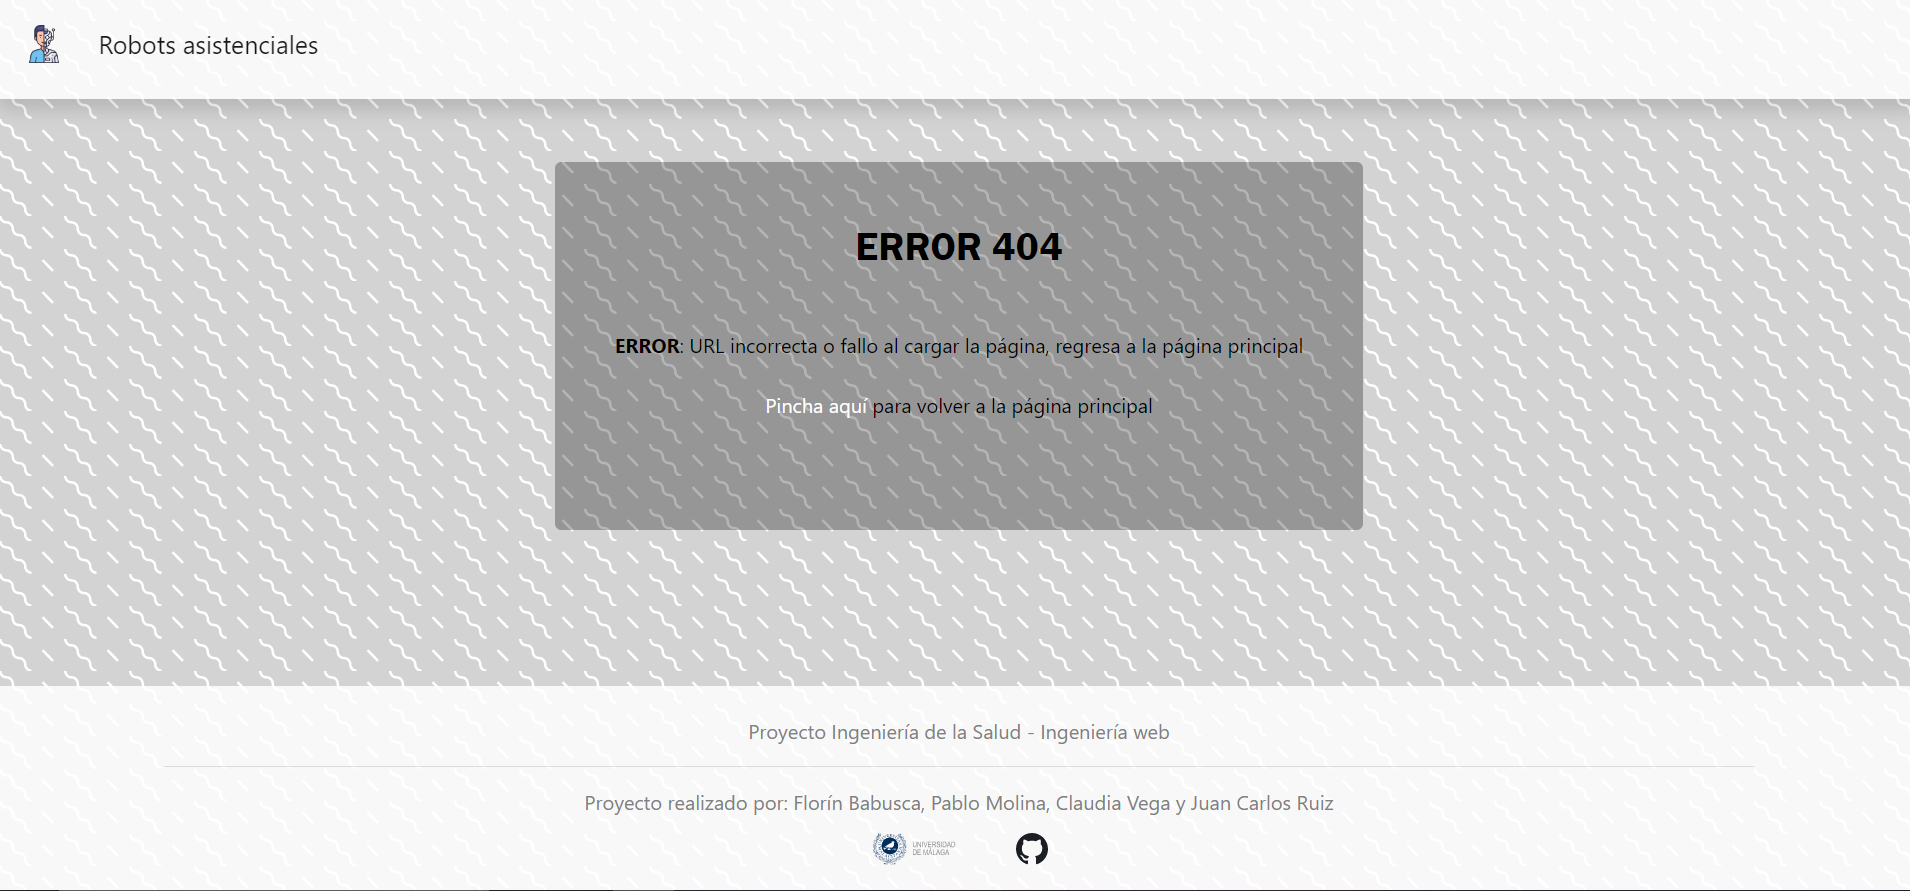
\includegraphics[width=1\textwidth]{images/error404.png}
	\caption{Error 404}
	\label{fig:UMLModel}
\end{figure}

%% incluir RNF 6 %%

\subsection{Requisitos no implementados}

No se ha podido realizar la implementación de los requisitos RF-3, RF-5, RF-8 y RNF-7 debido a la falta de tiempo y de recursos necesarios para su proceso. 

